% !TeX root = surprises.tex

%%%%%%%%%%%%%%%%%%%%%%%%%%%%%%%%%%%%%%%%%%%%%%%%%%%%%%%%%%%%%%%%

\selectlanguage{hebrew}

\chapter{האקסיומות של אוריגמי}\label{c.origami-axioms}

Origami, the art of paper folding, was developed several centuries ago in Japan and now has a worldwide following. In the late twentieth century the mathematical theory of origami was developed. Its foundation is a set of seven axioms, the 
\emph{Huzita–Hatori axioms}, named after Humiaki Huzita\index{Huzita, Humiaki} who formalized the first six axioms and Koshiro Hatori\index{Hatori, Koshiro} who found the seventh. Jacques Justin published all seven axioms several years before Huzita and Hatori, and Margherita P. Beloch\index{Beloch, Margherita P.} formulated the sixth axiom in 1936. Nevertheless, the axioms as known as the Huzita-Hatori axioms.

In a sequence of three chapters we will explore the mathematics of origami. This chapter presents the axioms, Chap.~\ref{c.origami-cube} connects origami with the roots of polynomials and Chap.~\ref{c.origami-constructions} shows that constructions with origami can solve problems that are impossible using a straightedge and compass.
 
This chapter contains a section for each of the seven axioms. Following a statement of an axiom and a diagram of the \emph{fold} it specifies, the equations of the fold and the points of intersection are developed using analytic geometry. A fold can also be defined as a \emph{geometric locus}\index{Geometric locus}, the set of all points satisfying some property. The term fold comes from the origami operation of folding a piece of paper, but here it is used to refer the geometric line that would be created by folding the paper.

Folds result in \emph{reflections}\index{Origami!reflection}. Given a point $p$, its reflection around a fold $l$ results in a point $p'$ such that $l$ is the perpendicular bisector of the line segment $\overline{pp'}$ (Fig.~\ref{f.origami-def}).

פעולות
\textbf{הקיפול}
מניח נקודות על נקודות או קווים, או קווים על קווים, כך שתנאים מסויימים מתקיימים. המונח קיפול בא מהפעולה באוריגמי של קיפול דף נייר, אבל כאן נשתמש בו עבור הקו הגיאומטרי שנוצר על ידי קיפול הדף. לפי ההגדרה, כתוצאה מקיפול נוצרים 
\textbf{שיקופים}.
נתונה נקודה 
$p$,
השיקוף שלה סביב הקיפול 
$l$,
הוא נקודה
$p'$,
כך ש-%
$l$
הוא האנך האמצעי של קטע הקו
$\overline{pp'}$:
\begin{center}

\begin{tikzpicture}
\coordinate (P1) at (2,2);
\coordinate (P1P) at (6,4);
\coordinate (mid) at (4,3);
\draw[rotate=30] (mid) rectangle +(8pt,8pt);
\coordinate (m1) at ($(P1)!.5!(mid)$);
\coordinate (m2) at ($(mid)!.5!(P1P)$);
\draw[thick] (m1) -- +(120:4pt);
\draw[thick] (m1) -- +(-60:4pt);
\draw[thick] (m2) -- +(120:4pt);
\draw[thick] (m2) -- +(-60:4pt);
\draw[thick] (P1) -- (P1P);
\draw[very thick,dashed] (4.7,1.6) -- node[very near end,right,yshift=4pt] {$l$} (3.5,4);
\fill (P1) circle(2pt) node[above left] {$p$};
\fill (P1P) circle(2pt) node[above left] {$p'$};
\fill (mid) circle(2pt);% node[below,xshift=-2pt,yshift=-8pt] {$p_i$};
\draw[very thick,dotted,->,bend right=50] (2,1.8) to (6,3.8);
\end{tikzpicture}
\end{center}

\selectlanguage{hebrew}


\section{אקסיומה 1}\label{s.ax1}


\textbf{אקסיומה:} 
נתונות שתי נקודות שונות
$p_1=(x_1,y_1)$, $p_2=(x_2,y_2)$,
קיים קיפול יחיד
$l$
העובר דרך שתיהן )איור~%
\ref{f.axiom1}(.
\begin{figure}[tb]
\begin{center}

\begin{tikzpicture}[scale=.9]
\draw[step=10mm,white!50!black,thin] (-1,-1) grid (8,6);
\draw[thick] (-1,0) -- (8,0);
\draw[thick] (0,-1) -- (0,6);
\foreach \x in {0,...,8}
  \node at (\x-.2,-.2) {\sm{\x}};
\foreach \y in {1,...,6}
  \node at (-.2,\y-.3) {\sm{\y}};
\coordinate (P1) at (2,2);
\coordinate (P2) at (6,4);
\draw[very thick,dashed] ($(P1)!-.75!(P2)$) -- node[very near end,below] {$l$} ($(P1)!1.5!(P2)$);
\fill (P1) circle(2pt) node[above left] {$p_1$};
\fill (P2) circle(2pt) node[above left] {$p_2$};

\draw[very thick,dotted,->,bend left=30] (2,5) to (4,1);
\end{tikzpicture}
\end{center}
\selectlanguage{hebrew}
\caption{אקסיומה 1}\label{f.axiom1}
\end{figure}

\textbf{פיתוח משוואת הקיפול:}
השיפוע של הקיפול הוא המנה של הפרשי הקואורינטות של
$p_1,p_2$,
ונקדות החיתוך עם ציר ה-%
$y$
מתקבלת מ-%
$p_1$:
\[
y - y_1 = \disfrac{y_2-y_1}{x_2-x_1}(x-x_1)\,.
\]
\textbf{דוגמה:}
נתונות הנקודות
$p_1=(2,2), p_2=(6,4)$,
המשוואה של 
$l$  היא:

\begin{eqn}
y-2&=&\disfrac{4-2}{6-2}(x-2)\\
y&=&\disfrac{1}{2}x+1\,.
\end{eqn}

%%%%%%%%%%%%%%%%%%%%%%%%%%%%%%%%%%%%%%%%%%%%%%%%%%%%%%%%%%%%%%%%

\selectlanguage{hebrew}



\section{אקסיומה 2}\label{s.ax2}


\textbf{אקסיומה:}
נתונות שתי נקודות שונות
$p_1=(x_1,y_1)$, $p_2=(x_2,y_2)$,
קיים קיפול יחיד 
$l$
המניח את
$p_1$
על
$p_2$:

%)איור~%
%\ref{f.axiom2}(.

%\begin{figure}
\begin{center}

\begin{tikzpicture}[scale=.9]
\draw[step=10mm,white!50!black,thin] (-1,-1) grid (8,6);
\draw[thick] (-1,0) -- (8,0);
\draw[thick] (0,-1) -- (0,6);
\foreach \x in {0,...,8}
  \node at (\x-.2,-.2) {\sm{\x}};
\foreach \y in {1,...,6}
  \node at (-.2,\y-.3) {\sm{\y}};
\coordinate (P1) at (2,2);
\coordinate (P2) at (6,4);
\coordinate (mid1) at ($(P1)!.5!(P2)$);
\coordinate (mid2) at ($(P1)!.5!(P2)+(-1,2)$);

\draw[rotate=30] (mid1) rectangle +(8pt,8pt);

\draw[very thick,dotted] (P1) -- (P2);
\draw[very thick,dashed] ($(mid1)!-1.4!(mid2)$) -- node[very near end,left,yshift=-12pt] {$l$} ($(mid1)!1.4!(mid2)$);
\fill (P1) circle(2pt) node[above left] {$p_1$};
\fill (P2) circle(2pt) node[above left] {$p_2$};

\draw[very thick,dotted,->,bend right=50] (2,1.8) to (6,3.8);
\end{tikzpicture}
\end{center}
%\caption{אקסיומה 2}\label{f.axiom2}
%\end{figure}


\textbf{פיתוח משוואת הקיפול:}
השיפוע של הקיפול
$l$
הוא ההופכי השלילי של השיפוע של הקו המחבר את
$p_1$
ו-%
$p_2$.
$l$
עובר דרך נקודת האמצע בין שתי הנוקדות:
\begin{equation}
y - \disfrac{y_1+y_2}{2} = -\disfrac{x_2-x_1}{y_2-y_1}\left(x-\disfrac{x_1+x_2}{2}\right)\,.\label{eq.midpoint1}
\end{equation}



\textbf{דוגמה:}
נתונות הנקודות
$p_1=(2,2), p_2=(6,4)$.
המשוואה של 
$l$
היא:

\begin{eqn}
y-\left(\disfrac{2+4}{2}\right)&=&-\disfrac{6-2}{4-2}\left(x-\left(\disfrac{2+6}{2}\right)\right)\\
y&=&-2x+11\,.
\end{eqn}


%%%%%%%%%%%%%%%%%%%%%%%%%%%%%%%%%%%%%%%%%%%%%%%%%%%%%%%%%%%%%%%%

\selectlanguage{hebrew}


\section{אקסיומה 3}\label{s.ax3}


\textbf{אקסיומה:}
נתונים שני קווים
$l_1$
ו-%
$l_2$,
קיים קיפול
$l$
המניח את
$l_1$ 
על
$l_2$.
%)איור~%
%\ref{f.axiom3}(.

%\begin{figure}[tb]
\begin{center}

\begin{tikzpicture}[scale=.9]
\draw[step=10mm,white!50!black,thin] (-1,-1) grid (8,7);
\draw[thick] (-1,0) -- (8,0);
\draw[thick] (0,-1) -- (0,7);
\foreach \x in {0,...,8}
  \node at (\x-.2,-.2) {\sm{\x}};
\foreach \y in {1,...,7}
  \node at (-.2,\y-.3) {\sm{\y}};
\coordinate (L1a) at (2,2);
\coordinate (L1b) at (4,6);
\draw[thick] (L1a) -- node[very near start,right,yshift=-4pt] {$l_1$} (L1b);
\draw[thick,dotted,name path=l1] ($(L1a)!-.75!(L1b)$) -- ($(L1a)!1.25!(L1b)$);
\coordinate (L2a) at (7,1);
\coordinate (L2b) at (4,4);
\draw[thick] (L2a) -- (L2b);
\draw[thick,dotted,name path=l2] ($(L2a)!-.3!(L2b)$) -- node[very near start,above,xshift=4pt,yshift=2pt] {$l_2$} ($(L2a)!2!(L2b)$);
\path [name intersections = {of = l1 and l2, by = {PM}}];
\fill (PM) circle(2pt) node[below left,xshift=-9pt,yshift=-7pt] {$p_i$};

\node[above right,xshift=10pt,yshift=4pt] at (PM) {$\alpha$};
\node[below right,xshift=10pt] at (PM) {$\alpha$};
\node[above left,xshift=-3pt,yshift=12pt] at (PM) {$\beta$};
\node[above right,xshift=-3pt,yshift=12pt] at (PM) {$\beta$};

\coordinate (B1a) at (0,4.13);
\coordinate (B1b) at (6,5.1);
\draw[very thick,dashed] ($(B1a)!-.15!(B1b)$) -- node[very near start,above] {$l_{f_1}$}  ($(B1a)!1.35!(B1b)$);

\coordinate (B2a) at (3,6.73);
\coordinate (B2b) at (4,.57);
\draw[very thick,dashed] ($(B2a)!-.05!(B2b)$) -- node[very near end,right,xshift=4pt,yshift=6pt] {$l_{f_2}$} ($(B2a)!1.25!(B2b)$);

\draw[very thick,dotted,->,bend right=50] (6,2.2) to (4.5,6.7);
\draw[very thick,dotted,->,bend left=50] (6.2,1.6) to (1.8,1.3);
\end{tikzpicture}
\end{center}
%\caption{אקסיומה 3}\label{f.axiom3}
%\end{figure}

\textbf{פיתוח משוואת הקיפול עבור קווים מקבילים:}
אם הקווים מקבילים, 
$l_1$
הוא
$y=mx+b_1$
ו-%
$l_2$
הוא
$y=mx+b_2$.
הקיפול הוא הקו המקביל ל-%
$l_1,l_2$ 
וחצי המרחק ביניהם:
\[
y=mx+\disfrac{b_1+b_2}{2}\,.
\]
\textbf{פיתוח משוואת הקיפול עבור קווים נחתכים:}
אם הקווים נחתכים,
$l_1$ 
הוא
$y=m_1x+b_1$
ו-%
$l_2$
הוא
$y=m_2x+b_2$.
$p_i=(x_i,y_i)$,
נקודת החיתוך שלהם, היא:

\begin{eqn}
m_1x_i+b_2&=&m_2x_i+b_2\\
x_i &=& \disfrac{b_2-b_1}{m_1-m_2}\\
y_i &=&m_1x_i+b_1\,.
\end{eqn}



\textbf{דוגמה:}
נתון הקו
$l_1$
שהמשוואה שלו הוא
$y\!=\!2x-2$,
והקו
$l_2$
שהמשוואה שלו הוא
$y\!=\!-x+8$.
נקודת החיתוך שלהם היא:

\begin{eqn}
x_i&=&\disfrac{8-(-2)}{2-(-1)}=\disfrac{10}{3}\approx 3.33\\
y_i &=& 2\cdot\disfrac{10}{3}-2=\disfrac{14}{3}\approx 4.67\,.
\end{eqn}

\textbf{פיתוח משוואת השיפוע של חוצה הזווית:}
שני קווים יוצרים שני זוגות של זוויות קודקודיות. הקיפולים הם חוצי הזווית שלהן.
אם הזווית של
$l_1$
יחסית לציר ה-%
$x$
היא
$\theta_1$ 
והזווית של 
$l_2$
יחסית לציר ה-%
$x$
היא
$\theta_2$,
אזי קיפול הוא הקו היוצר זווית של:
\[
\theta_b=
\theta_1+\disfrac{\theta_2-\theta_1}{2}=
\disfrac{\theta_1}{2}+\disfrac{\theta_2}{2}=
\disfrac{\theta_1+\theta_2}{2}
\]
יחסית לציר ה-%
$x$:

\begin{center}

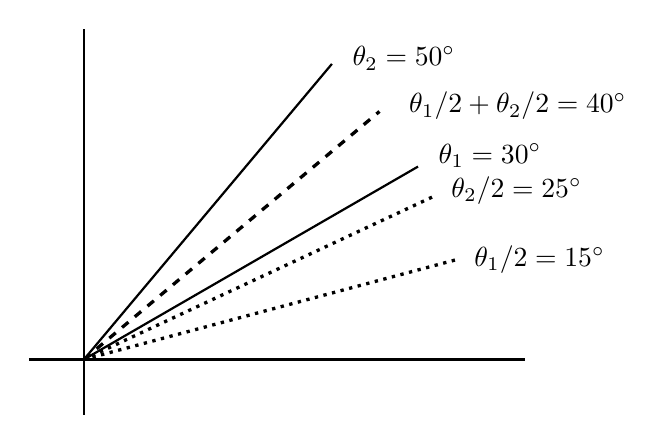
\begin{tikzpicture}[scale=.7]
\draw[thick] (-1,0) -- (8,0);
\draw[thick] (0,-1) -- (0,6);
  
\draw[thick] (0,0) -- +(30:7)
  node[xshift=26pt,yshift=4pt] {$\theta_1=30^\circ$};
\draw[thick] (0,0) -- +(50:7)
  node[xshift=26pt,yshift=2pt] {$\theta_2=50^\circ$};
\draw[very thick,dotted] (0,0) -- +(15:7)
  node[xshift=30pt,yshift=0pt] {$\theta_1/2=15^\circ$};
\draw[very thick,dotted] (0,0) -- +(25:7)
  node[xshift=30pt,yshift=2pt] {$\theta_2/2=25^\circ$};
\draw[very thick,dashed] (0,0) -- +(40:7)
  node[xshift=50pt,yshift=2pt] {$\theta_1/2+\theta_2/2=40^\circ$};
\end{tikzpicture}
\end{center}
$\tan\theta_1=m_1$
ו-%
$\tan\theta_2=m_2$
נתונים ו-%
$m_b$,
השיפוע של חוצה הזווית, הוא:
\[
m_b=\tan\theta_b=\tan\disfrac{\theta_1+\theta_2}{2}\,.
\]
פיתוח המשוואה מחייב שימוש בשוויונות הטריגונומטריות:

\begin{eqn}
\tan(\phi_1+\phi_2)&=& \disfrac{\tan\phi_1+\tan\phi_2}{1-\tan\phi_1\tan\phi_2}\\
\tan \disfrac{\phi}{2}&=& \disfrac{-1\pm\sqrt{1+\tan^2\phi}}{\tan \phi}\,.
\end{eqn}
תחילה נמצא את
$m_s$,
השיפוע של
$\theta_1+\theta_2$:
\[
m_s=\tan(\theta_1+\theta_2)= \disfrac{m_1+m_2}{1-m_1m_2}\,.
\]
אחר כך נמצא את 
$m_b$,
השיפוע של חוצה הזווית:

\begin{eqn}
m_b&=& \tan\disfrac{\theta_1+\theta_2}{2}\\
&=&\disfrac{-1\pm\sqrt{1+\tan^2(\theta_1+\theta_2)}}{\tan (\theta_1+\theta_2)}\\
&=&\disfrac{-1\pm\sqrt{1+m_s^2}}{m_s}\,.
\end{eqn}



\textbf{דוגמה:}
נתונים הקווים
$y=2x-2$
ו-%
$y=-x+8$,
השיפוע של חוצה הזווית הוא:

\begin{eqn}
m_s&=&\disfrac{2+(-1)}{1-(2 \cdot -1)}=\disfrac{1}{3}\\
m_b&=&\disfrac{-1\pm\sqrt{1+(1/3)^2}}{1/3}=-3\pm \sqrt{10}\approx -6.16,\; 0.162\,.
\end{eqn}



\textbf{פיתוח משוואת הקיפול:}
נפתח את המשוואה של
$l_{f_1}$
עם השיפוע החיובי
$-3+ \sqrt{10}$.
חישבנו לעיל את הקואורדינטות של נקודת החיתוך של הקווים 
$m_i=\left(\disfrac{10}{3},\disfrac{14}{3}\right)$.
נקודת החיתוך של 
$l_{f_1}$
עם ציר ה-%
$y$
היא:

\begin{eqn}
\disfrac{14}{3} &=& (-3+\sqrt{10}) \cdot \disfrac{10}{3} + b\\ b&=&\disfrac{44-10\sqrt{10}}{3}\\
y&=& (-3+\sqrt{10})x + \disfrac{44-10\sqrt{10}}{3}\approx 0.162x+4.13\,.
\end{eqn}

%%%%%%%%%%%%%%%%%%%%%%%%%%%%%%%%%%%%%%%%%%%%%%%%%%%%%%%%%%%%%%%%

\section{אקסיומה 4}\label{s.ax4}


\textbf{אקסיומה:}
נתונים נקודה
$p_1=(x_1,x_2)$
וקו
$l_1$,
קיים קיפול יחיד
$l$
הניצב ל-%
$l_1$
שעובר דרך
$p_1$.
)איור~%%
%\ref{f.axiom4}(.

%\begin{figure}[tb]
\begin{center}

\begin{tikzpicture}[scale=.9]
\draw[step=10mm,white!50!black,thin] (-1,-1) grid (8,7);
\draw[thick] (-1,0) -- (8,0);
\draw[thick] (0,-1) -- (0,7);
\foreach \x in {0,...,8}
  \node at (\x-.2,-.2) {\sm{\x}};
\foreach \y in {1,...,7}
  \node at (-.2,\y-.3) {\sm{\y}};
\coordinate (L1a) at (2,0);
\coordinate (L1b) at (5,6);
\draw[thick] (L1a) -- node[very near start,right,yshift=-4pt] {$l_1$} ($(L1a)!1.15!(L1b)$);
\fill (2,6) circle (2pt) node[above right] {$p_1$};
\draw[thick,dashed] (0,7) -- node[very near end,above right] {$l$} (8,3);
\coordinate (intersection) at (4.4,4.8);
\draw[rotate=-30] (intersection) rectangle +(8pt,8pt);

\draw[very thick,dotted,->,bend left=50] (5.4,6.3) to (3.7,3);
\end{tikzpicture}
\end{center}
%\caption{אקסיומה 4}\label{f.axiom4}
%\end{figure}

\textbf{פיתוח משוואת הקיפול:}
המשוואה של הקו
$l_1$
היא
$y = m_1x + b_1$.
$l$
ניצב ל-%
$l_1$
לכן השיפוע שלו הוא
$-\disfrac{1}{m_1}$.
הקו עובר דרך
$p_1$
ונוכל לחשב את המשוואה שלו:

\begin{eqn}
y_1&=&-\disfrac{1}{m} x_1 + b\\
b&=& \disfrac{(my_1+x_1)}{m}\\
y&=&-\disfrac{1}{m} x +\disfrac{(my_1+x_1)}{m}\,.
\end{eqn}



\textbf{דוגמה:}
נתונה הנקודה
$p_1=(2,6)$
ונתון הקו
$l_1$
שהמשוואה שלו הוא
$y=2x-4$.
המשוואה של הקיפול
$l$
היא:
\[
y=-\disfrac{1}{2}x + \disfrac{2\cdot 6 + 2}{2}=-\disfrac{1}{2}x + 7\,.
\]

%%%%%%%%%%%%%%%%%%%%%%%%%%%%%%%%%%%%%%%%%%%%%%%%%%%%%%%%%%%%%%%%

\selectlanguage{hebrew}



\section{אקסיומה 5}\label{s.ax5}


\textbf{אקסיומה:} 
נתונות נקודות
$p_1=(x_1,y_1)$, $p_2=(x_2,y_2)$
ונתון קן
$l_1$,
קיים קיפול
$l$
המניח את
$p_1$
מעל
$l_1$
והעובר דרך
$p_2$.
%)איור~%
%\ref{f.axiom5}(.

%\begin{figure}[tb]
\begin{center}

\begin{tikzpicture}[scale=.9]
\draw[step=10mm,white!50!black,thin] (-1,-1) grid (9,9);
\draw[thick] (-1,0) -- (9,0);
\draw[thick] (0,-1) -- (0,9);
\foreach \x in {0,...,9}
  \node at (\x-.2,-.2) {\sm{\x}};
\foreach \y in {1,...,9}
  \node at (-.2,\y-.3) {\sm{\y}};
\coordinate (L1a) at (0,3);
\coordinate (L1b) at (8,-1);
\draw[thick] (L1a) -- node[near end,below right,xshift=8pt,yshift=-8pt] {$l_1$} (L1b);
\coordinate (P1) at (2,8);
\fill (P1) circle (2pt) node[above left] {$p_1$};
\coordinate (P2) at (4,4);
\fill (P2) circle (2pt) node[above left,yshift=4pt] {$p_2$};
\draw[thick,dotted,name path=L1] (8,-1) -- (-1,3.5);
\node[very thick,dotted,draw, name path = circle] at (P2)
    [circle through = (P1)] {};

\path [name intersections = {of = circle and L1, by = {P1P,P1PP}}];
\fill (P1P) circle (2pt) node[above left,xshift=-2pt,yshift=4pt] {$p_1'$};
\fill (P1PP) circle (2pt) node[above left,yshift=6pt] {$p_1''$};

\coordinate (f1) at (0,6);
\draw[thick,dashed] ($(f1)!-.25!(P2)$) -- node[very near end,above] {$l_{f_2}$} ($(f1)!2.25!(P2)$);
\coordinate (f2) at (0,2);
\draw[thick,dashed] ($(f2)!-.25!(P2)$) -- node[very near end,below,yshift=-2pt] {$l_{f_1}$} ($(f2)!2.25!(P2)$);

\draw[very thick,dotted,->,bend left=50] (2.2,7.8) to (-.2,3.2);
\draw[very thick,dotted,->,bend left=50] (2.4,7.85) to (6.1,.2);
\end{tikzpicture}
\end{center}
%\caption{}\label{f.axiom5}
%\end{figure}

עבור זוג נקודות נתון וקו נתון, יכולים להיות אפס, אחד או שני קיפולים.

\textbf{פיתוח משוואות עבור השיקופים:}
נסמן ב-%
$l$
את הקיפול העובר דרך
$p_2$,
ונסמן ב-%
$p_1'$
את השיקוף של
$p_1$
מסביב ל-%
$l$.
האורך של
$\overline{p_1p_2}$
שווה לאורך של
$\overline{p_2p_1}'$.
המקום הגיאומטרי של נקודות הנמצאות במרחק
$\overline{p_1p_2}$
מ-%
$p_2$
הוא המעגל שמרכזו
$p_2$
והרדיוס שלו הוא
$\overline{p_1p_2}$. 
נקודות החיתוך של מעגל זה עם הקו
$l_1$
הן המקומות האפשריים עבור
$p_1'$.
המשוואה של הקו
$l_1$
היא
$y=m_1x + b_1$.
המשוואה של המעגל שמרכזו
$p_2$
עם רדיוס
$\overline{p_1p_2}$
היא:
\[
(x-x_2)^2 + (y-y_2)^2 = r^2\,.
\]



נציב את המשוואה של הקו לתוך המשוואה של המעגל:

\begin{eqn}
(x-x_2)^2+((m_1x+b_1)-y_2)^2&=&r^2\\
(x-x_2)^2+(m_1x+(b_1-y_2))^2&=&r^2\,,
\end{eqn}



ונקבל משוואה ריבועית עבור קואורדינטות ה-%
$x$
של נקודות החיתוך האפשריות:
\begin{equation}
x^2(1+m_1^2) \,+\, 2(-x_2+m_1(b-y_2))x \,+\, (x_2^2 + (b_1-y_2)^2-r^2)=0\,.\label{eq.intersections}
\end{equation}




למשוואה ריבועית יש לכל היותר שני פתרונות
$x_1',x_1''$,
ונחשב את 
$y_1',y_1''$
מ-%
$y=m_1x+b_1$.
נקודות השיקוף הן
$p_1'=(x_1',y_1'), p_1''=(x_1'',y_1'')$.



\textbf{דוגמה:}
נתונות הנקודות
$p_1=(2,8)$,
$p_2=4,4)$,
ונתון הקו
$l_1$ 
שהמשוואה שלו היא
$y=-\disfrac{1}{2}x +3$.
משוואת המעגל היא:
\[
(x-4)^2 + (y-4)^2 = r^2=(4-2)^2+(4-8)^2=20\,.
\]
נציב את המשוואה של הקו לתוך המשוואה של המעגל ונפשט כדי לקבל משוואה ריבועית עבור קואורדינטות ה-%
$x$
של נקודות החיתוך )או השתמשו במשוואה
~\ref{eq.intersections}(.

\begin{eqn}
(x-4)^2 + \left(\left(-\disfrac{1}{2}x+3\right)-4\right)^2&=&20\\
\disfrac{5}{4}x^2-7x-3 &=&0\\
5x^2 -28x -12&=&0\\
(5x+2)(x-6)&=&0\,.
\end{eqn}
שתי נקודות חיתוך הן:
\[
p_1'=\left(-\disfrac{2}{5},\disfrac{16}{5}\right) = (-0.4,3.2)\,,\quad p_1''=(6,0)\,.
\]
\textbf{פיתוח המשוואות של הקיפולים:}
הקיפולים יהיו האנכים האמצעיים של
$\overline{p_1p_1'}$
ו-%
$\overline{p_1p_1''}$.
המשוואה של אנך אמצעי נתונה על ידי משוואה%
~\ref{eq.midpoint1},
שנעתיק כאן עבור
$p_1'$:
\begin{equation}
y - \disfrac{y_1+y_1'}{2} = -\disfrac{x_1'-x_1}{y_1'-y_1}\left(x-\disfrac{x_1+x_1'}{2}\right)\,.\label{eq.midpoint2}
\end{equation}

\textbf{דוגמה:}
נתונות הנקודות
$p_1=(2,8)$,
$p_1'=\left(-\disfrac{2}{5},\disfrac{16}{5}\right)$,
משוואת הקיפול של
$l_{f_1}$
היא:

\begin{eqn}
y-\disfrac{8+(16/5)}{2}&=&-\disfrac{(-2/5)-2}{(16/5)-8}\left(x-\disfrac{2+\left(-2/5\right)}{2}\right)\\
y&=&-\disfrac{1}{2}x+6\,.
\end{eqn}



נתונות הנקודות עבור
$p_1=(2,8)$,
$p_1''=(6,0)$,
משוואת הקיפול של
$l_{f_2}$ 
היא:

\begin{eqn}
y-\disfrac{8+0}{2}&=&-\disfrac{6-2}{0-8}\left(x-\disfrac{2+6}{2}\right)\\
y&=&\disfrac{1}{2}x+2\,.
\end{eqn}

%%%%%%%%%%%%%%%%%%%%%%%%%%%%%%%%%%%%%%%%%%%%%%%%%%%%%%%%%%%%%%%%

\selectlanguage{hebrew}



\section{אקסיומה 6}\label{s.ax6}

\textbf{אקסיומה:}                         
נתונות שתי נקודות
$p_1$
ו-%
$p_2$
ונתונים שני קווים
$l_1$
ו-%
$l_2$,
קיים קיפול
$l$
המניח את 
$p_1$
על ל-%
$l_1$
ו-%
$p_2$
על ל-%
$l_2$.
%)איור~%
%\ref{f.axiom6}(.

%\begin{figure}[tb]
\begin{center}

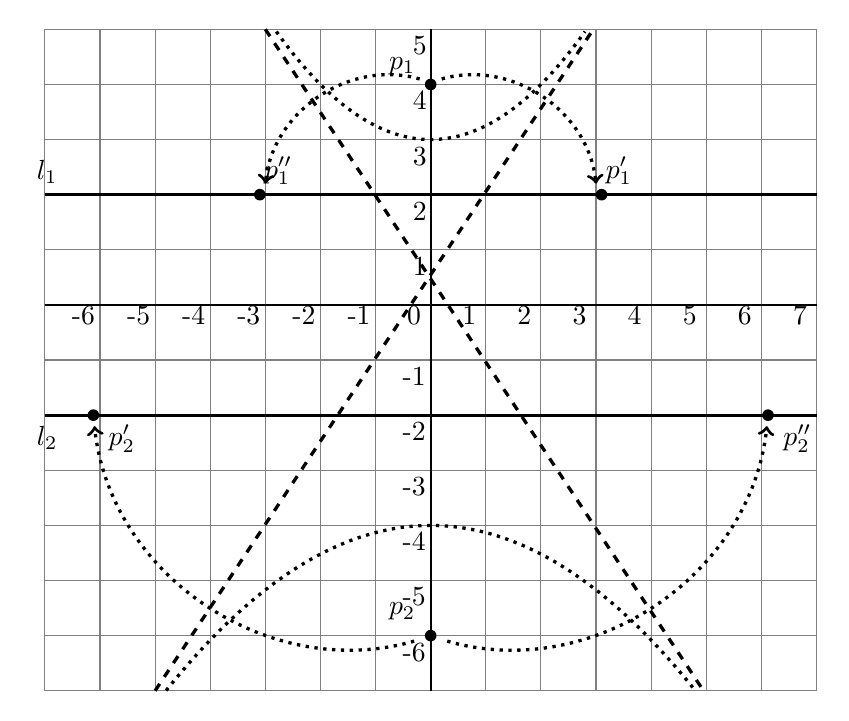
\begin{tikzpicture}[scale=.7]
\draw[step=10mm,white!50!black,thin] (-7,-7) grid (7,5);
\draw[thick] (-7,0) -- (7,0);
\draw[thick] (0,-7) -- (0,5);
\foreach \x in {-6,...,7}
  \node at (\x-.3,-.2) {\sm{\x}};
\foreach \y in {1,...,5}
  \node at (-.2,\y-.3) {\sm{\y}};
\foreach \y in {-6,...,-1}
  \node at (-.3,\y-.3) {\sm{\y}};
  
\coordinate (P1) at (0,4);
\fill (P1) circle (3pt) node[above left,xshift=-2pt] {$p_1$};
\coordinate (P2) at (0,-6);
\fill (P2) circle (3pt) node[above left,xshift=-2pt,yshift=2pt] {$p_2$};

\coordinate (P1P) at (3.1,2);
\fill (P1P) circle (3pt) node[above right,xshift=-2pt] {$p_1'$};
\coordinate (P2P) at (-6.12,-2);
\fill (P2P) circle (3pt) node[below right,xshift=2pt] {$p_2'$};

\coordinate (P1PP) at (-3.1,2);
\fill (P1PP) circle (3pt) node[above right,xshift=-2pt] {$p_1''$};
\coordinate (P2PP) at (6.12,-2);
\fill (P2PP) circle (3pt) node[below right,xshift=2pt] {$p_2''$};

\draw[very thick] (-7,2) -- node[very near start,above,xshift=-34pt] {$l_1$} (7,2);
\draw[very thick] (-7,-2) -- node[very near start,below,xshift=-34pt] {$l_2$} (7,-2);

\draw[domain=-4.8:4.8,samples=50,very thick,dotted] plot (\x,{-.13*\x*\x-4});
\draw[domain=-2.8:2.8,samples=50,very thick,dotted] plot (\x,{.25*\x*\x+3});

\draw[very thick,dashed] (-5,-7) -- (2.95,5);
\draw[very thick,dashed] (-3,5) -- (4.95,-7);

\draw[very thick,dotted,->,bend left=50] (.2,4.1) to (3,2.2);
\draw[very thick,dotted,->,bend left=50] (-.3,-6.1) to (-6.1,-2.2);

\draw[very thick,dotted,->,bend right=50] (-.2,4.1) to (-3,2.2);
\draw[very thick,dotted,->,bend right=50] (.3,-6.1) to (6.1,-2.2);
\end{tikzpicture}
\end{center}
%\caption{אקסיומה 6}\label{f.axiom6}
%\end{figure}

עבור נקודות נתונות וקווים נתונים יכולים להיות אפס, אחד, שניים או שלושה קיפולים.
% איורים~
%\ref{f.two-para-1}, \ref{f.two-para-2}
%האיור בסעיף~%
%\ref{s.parabola}
%מראה דוגמאות גרפיות לארבעת האפשרויות.

קיפול המניח את 
$p_i$
על
$l_i$
הוא קו שמרחקו ל-%
$p_i$
שווה למרחקו ל-%
$l_i$.
המקום הגיאומטרי של נקודות שהן במרחק שווה מנקודה
$p_i$
ומקו
$l_i$
הוא פרבולה עם מוקד 
\L{(focus)}
$p_i$
ומדריך
\L{(directrix)}
$l_i$.
קיפול הוא קו המשיק לפרבולה )סעיף~%
\ref{s.parabola}(.
כדי שהקיפול יניח בו-זמנית את 
$p_1$
על ל-%
$l_1$
ו-%
$p_2$
על ל-%
$l_2$,
הוא חייב להיות משיק משותף לשתי הפרבולות.

המשוואה עבור פרבולה שרירותית מסובכת ולכן נגביל את הדיון לפרבולה שציר ה-%
$y$
הוא ציר הסמטריה. נביא גם דוגמה עם פרבולה שציר הסמטריה שלה הוא ציר ה-%
$x$.

\selectlanguage{hebrew}


\subsection{פיתוח הנקודה של הקיפול}

התיאור שלהלן מתייחס לאיור~%
\ref{f.parabola}.
הנקודה
$(0,f)$
היא מוקד של פרבולה עם מדריך
$y=d$.
נגדיר
$p=f-d$,
האורך 
)$\pm$(
של קטע הקו בין המוקד למדריך. אם הקודקוד 
\L{(vertex)}
נמצא על ציר ה-%
$x$,
המשוואה של הפרבולה היא
$y=\disfrac{x^2}{2p}$.
כדי להזיז את הפרבולה על ציר ה-%
$y$,
כך שהקודקוד שלה היא
$(0,h)$,
יש להוסיף 
$h$
למשוואת הפרבולה:
$y=\disfrac{x^2}{2p}+h$.
\begin{figure}[tb]
\begin{center}

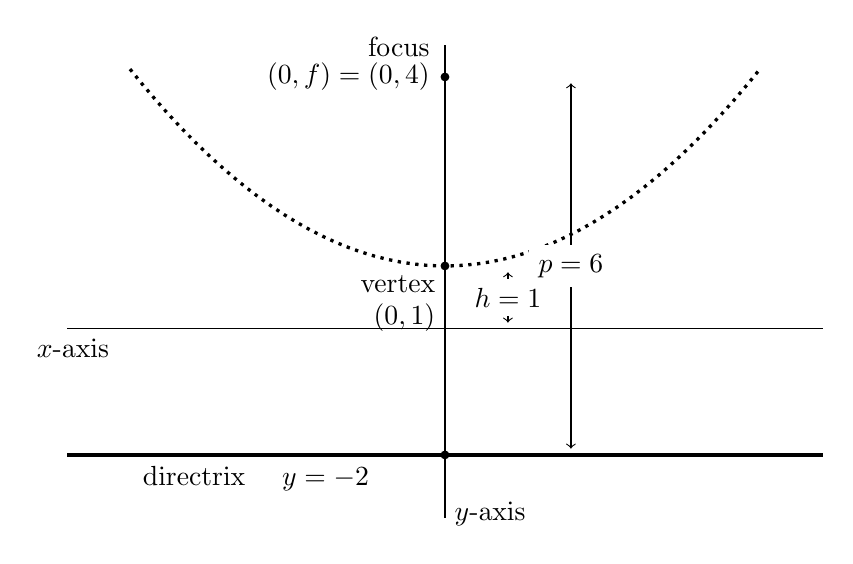
\begin{tikzpicture}[scale=.8]
\draw (-6,0) -- node[very near start,below,xshift=-32pt] {$x$-axis}(6,0);
\draw (0,-3) -- node[very near start,right,yshift=-20pt] {$y$-axis}(0,4.5);
\draw[very thick] (-6,-2) -- node[near start,below] {directrix $\quad y=-2$} (6,-2);

%\draw (-6,0) -- node[very near start,below,xshift=-32pt] {$x$-\R{ציר}}(6,0);
%\draw (0,-3) -- node[very near start,right,yshift=-20pt] {$y$-\R{ציר}}(0,4.5);
%\draw[very thick] (-6,-2) -- node[near start,below] {\R{מדריך} $\quad y=-2$} (6,-2);

\draw[domain=-5:5,samples=50,very thick,dotted] plot (\x,{\x*\x/8+1});
\coordinate (F) at (0,4);
\fill (F) circle (2pt) node[left,xshift=-2pt,yshift=0pt] {$(0,f)=(0,4)$} node[above left,xshift=-2pt,yshift=4pt] {focus};
%\fill (F) circle (2pt) node[left,xshift=-2pt,yshift=0pt] {$(0,f)=(0,4)$} node[above left,xshift=-2pt,yshift=4pt] {\R{מוקד}};
\fill (0,-2) circle (2pt);
\fill (0,1) circle (2pt) node[below left] {vertex} node[below left,yshift=-10pt] {$(0,1)$};
%\fill (0,1) circle (2pt) node[below left] {\R{קודקוד}} node[below left,yshift=-10pt] {$(0,1)$};
\draw[<->] (2,-1.9) -- node[fill=white] {$p=6$} +(0,5.8);
\draw[<->] (1,.1) -- node[fill=white] {$h=1$} +(0,.8);
\end{tikzpicture}
\end{center}
\selectlanguage{hebrew}
\caption{הגדרת הפרבולה: מוקד, מדריך, קודקוד}\label{f.parabola}
\end{figure}
נגדיר
$a=2ph$
כך שמשוואת הפרבולה היא:



\begin{eqn}
y&=&\disfrac{x^2}{2p}+\disfrac{a}{2p}\\
x^2-2py+a&=&0\,.
\end{eqn}
עבור הפרבולה באיור~%
\ref{f.parabola}
המשוואה היא:

\begin{eqn}
x^2-2\cdot 6\,y + 2\cdot 6 \cdot 1&=&0\\
x^2-12y +12&=&0\,.
\end{eqn}


נציב את המשוואה של קו 
\textbf{שרירותי}
$y=mx+b$
במשוואה עבור הפרבולה ונקבל משוואה עבור נקודות החיתוך של הקו והפרבולה:

\begin{eqn}
x^2-2p(mx+b)+a&=&0\\
x^2+(-2mp)x+(-2pb+a)&=&0\,.
\end{eqn}



הקו יהיה משיק לפרבולה אם ורק אם למשוואה ריבועית זו קיים 
\textbf{בדיוק}
פתרון אחד אם ורק אם הדיסקרימננטה 
)\L{discriminant}(
היא אפס:
\begin{eqnlabels}
(-2mp)^2\:-\:4\cdot 1\cdot (-2pb+a)&=&0\\
m^2p^2+2pb-a&=&0\,.\label{eq.disc}
\end{eqnlabels}



משוואה זו עם המשתנה 
$m$ 
היא המשוואה ריבועית עבור השיפועים של המשיקים לפרבולה. קיימים אינסוף משיקים כי עבור כל 
$m$,
קיים
$b$
שגורם למשיק לזוז למעלה או למטה.%
\footnote{\R{פרט כמובן עבור קו המקביל לציר הסמטריה}.}
כדי למצוא את המשיקים המשותפים לשתי הפרבולות, יש לפתור את המשוואות של שתי הפרבולות, משוואות עם שני משתנים
$m$
ו-%
$b$.

%%%%%%%%%%%%%%%%%%%%%%%%%%%%%%%%%%%%%%%%%%%%%%%%%%%%%%%%%%%%%%%%

\selectlanguage{hebrew}


\subsection{דוגמאות לאקסיומה 6}

\textbf{פרבולה 1:}
מוקד
$(0,4)$,
מדריך
$y=2$,
קודקוד
$(0,3)$.


$p=4-2=2$, $a=2\cdot 2\cdot 3=12$.
משוואת הפרבולה היא:
\[
x^2-2\cdot 2y +12=0\,.
\]
נציב לתוך משוואה%
~\ref{eq.disc}
ונפשט:
\[
m^2+b-3=0\,.
\]
\textbf{פרבולה 2:}
מוקד
$(0,-4)$,
מדריך
$y=-2$,
קודקוד
$(0,-3)$.

$p=-4-(-2)=-2$, $a=2\cdot -2\cdot -3=12$.
משוואת הפרבולה היא:
\[
x^2-2\cdot (-2)y+12=0\,.
\]
נציב לתוך משווארה%
~\ref{eq.disc}
ופשט:
\[
m^2-b-3=0\,.
\]
הפתרונות של שתי המשוואות:

\begin{eqn}
m^2+b-3&=&0\\
m^2-b-3&=&0\,,
\end{eqn}


הם
$m=\pm\sqrt{3}\approx \pm 1.73$
ו-%
$b=0$.
המשיקים המשותפים שהם הקיפולים הם:
\[
y=\sqrt{3}x\,,\quad y=-\sqrt{3}x\,.
\]
%%%%%%%%%%%%%%%%%%%%%%%%%%%%%%%%%%%%%%%%%%%%%%%%%%%%%%%%%%%%%%%%



\textbf{פרבולה 1:}
ללא שינוי, המשוואה היא:
\[
m^2+b-3=0\,.
\]
\textbf{פרבולה 2:}
מוקד
$(0,-6)$,
מדריך
$y=-2$,
קודקוד
$(0,-4)$.

$p=-6-(-2)=-4$, $a=2\cdot -4\cdot -4=32$.
משוואת הפרבולה היא:
\[
x^2-2\cdot (-4)y +32=0\,.
\]
נציב לתוך משווארה%
~\ref{eq.disc}
ונפשט:
\[
2m^2-b-4=0\,.
\]
הפתרונות של שתי המשוואות:

\begin{eqn}
m^2+b-3&=&0\\
2m^2-b-4&=&0\,,
\end{eqn}
הם
$m=\pm\sqrt{\disfrac{7}{3}}\approx \pm 1.53$
ו-%
$b=\disfrac{2}{3}$.
יש שני משיקים משותפים שהם קיפולים:
\[
y=\sqrt{\disfrac{7}{3}}x+\disfrac{2}{3}\,,\quad y=-\sqrt{\disfrac{7}{3}}x+\disfrac{2}{3}\,.
\]
%%%%%%%%%%%%%%%%%%%%%%%%%%%%%%%%%%%%%%%%%%%%%%%%%%%%%%%%%%%%%%%%


\textbf{פרבולה 1:}
ללא שינוי, המשוואה היא:
\[
m^2+b-3=0\,.
\]
\textbf{פרבולה 2:}
פרבולה שציר הסמטריה שלה הוא ציר ה-%
$x$.
מוקד
$(4,0)$,
מדריך
$x=2$,
קודקוד
$(3,0)$.
$p=4-2=2$, $a=2\cdot 2\cdot 3=12$.
משוואת הפרבולה היא:
\[
y^2-4x+12 = 0\,.
\]
שימו לב שזו משוואה עם 
$x$
ו-%
$y^2$
במקום
$x^2$
ו-%
$y$,
כך שלא ניתן להשתמש במשוואה%
~\ref{eq.disc}
ונצטרך לפתח את משוואות מחדש.

נציב את המשוואה של הקו:

\begin{eqn}
(mx+b)^2-4x+12&=&0\\
m^2x^2+(2mb-4)x+(b^2+12)&=&0\,
\end{eqn}
נשווה את הדיסקרימננטה לאפס ונפשט:

\begin{eqn}
(2mb-4)^2\:-\:4m^2(b^2+12)&=&0\\
-3m^2-mb+1&=&0\,.
\end{eqn}
אם ננסה לפתור את שתי המשוואות:

\begin{eqn}
m^2+b-3&=&0\\
-3m^2-mb+1&=&0\,,
\end{eqn}
נקבל משוואה 
\textbf{ממעלה שלוש}
במשתנה
$m$:
\begin{equation}
m^3-3m^2-3m+1=0\,.\label{eq.cubic}
\end{equation}



למשוואה ממעלה שלוש יש לפחות פתרון ממשי אחד ולכל היותר שלושה פתרונות ממשיים, לכן יכול להיות אחד, שניים או שלשה משיקים משותפים. הנוסחה למציאת פתרונות למשוואה ממעלה שלוש די מסובכת, לכן השתמשתי במחשבון באינטרנט וקיבלתי שלושה פתרונות:
\[
m=3.73\,, \;m=-1\,, \; m=0.27\,.
\]
אם נבחר
$m=0.27$, $b=3-m^2=2.93$,
משוואת הקיפול היא:
\[
y=0.27x+2.93\,.
\]
מהצורה של המשוואה%
~\ref{eq.cubic},
נוכל לנחש ש-%
$1$
או
$-1$
הוא פתרון:

\begin{eqn}
1^3-3\cdot 1^2-3\cdot 1+1&=&-4\\
(-1)^3-3\cdot (-1)^2-3\cdot(-1)+1&=&0\,.
\end{eqn}


נחלק את המשוואה%
~\ref{eq.cubic}
ב-%
$m-(-1)=m+1$
ונקבל משוואה ריבועית
$m^2-4m+1$
ששורשיה הם
$2\pm\sqrt{3}\approx 3.73, 0.27$.


%%%%%%%%%%%%%%%%%%%%%%%%%%%%%%%%%%%%%%%%%%%%%%%%%%%%%%%%%%%%%%%%
\selectlanguage{hebrew}


\subsection{פיתוח המשוואות של השיקופים}

נחשב את  
$p_1'=(x_1',y_1')$,
השיקוף של
$p_1=(x_1,y_1)$
מסביב למשיק
$l_t$
שהמשוואה שלה היא
$y=m_tx+b_t$.
)החישוב דומה עבור כל משיק ועבור
$p_2$.(
נמצא את הקו
$l_p$
עם המשוואה
$y=m_px+b_p$
שניצב ל-%
$l_t$
ועובר דרך
$p_1$:

\begin{eqn}
y&=&-\disfrac{1}{m_t}x+b_p\\
y_1&=&-\disfrac{1}{m_t}x_1+b_p\\
y&=&\disfrac{-x}{m_t}+\left(y_1+\disfrac{x_1}{m_t}\right)\,.
\end{eqn}



כעת נמצא את נקודת החיתוך 
$p_t=(x_t,y_t)$
של
$l_t$
ו-%
$l_p$:




\begin{eqn}
m_tx_t+b_t&=&\disfrac{-x_t}{m_t}+\left(y_1+\disfrac{x_1}{m_t}\right)\\
%x_t&=&\disfrac{\left(y_1+\disfrac{x_1}{m_t}-b_t\right)}{\left(m_t+\disfrac{1}{m_t}\right)}\\
x_t&=& \disfrac{m_t(y_1-b_t)+x_1}{m_t^2+1}\\
y_t&=&m_tx_t+b_t\,.
\end{eqn}



ניתן למצוא את השיקוף
$p_1'$
כי נקודת החיתוך
$p_t$
היא נקודת האמצע בין
$p_1$
לבין
$p_1'$:




\begin{eqn}
x_t&=&\disfrac{x_1+x_1'}{2}\,,\quad y_t=\disfrac{y_1+y_1'}{2}\\
x_1'&=&2x_t-x_1\,,\quad y_1'=2y_t-y_1\,.
\end{eqn}



\textbf{דוגמה:}
נתון
$p_1=(0,4)$
ו-%
$l_1$
עם המשוואה
$y=\sqrt{3}x$:

\begin{eqn}
%x_t&=&\disfrac{\left(4+\disfrac{0}{\sqrt{3}}-0\right)}{\left(\sqrt{3}+\disfrac{1}{\sqrt{3}}\right)}=\sqrt{3}\\
x_t&=&\disfrac{\sqrt{3}(4-0)+0}{(\sqrt{3})^2+1}=\sqrt{3}\\
y_t&=&\sqrt{3}\sqrt{3}+0=3\\
x_1'&=&2x_t-x_1=2\sqrt{3}-0=2\sqrt{3}\approx 3.46\\
y_1'&=&2y_t-y_1=2\cdot 3 - 4 = 2\,.
\end{eqn}

\selectlanguage{hebrew}


\subsection{משיקים לפרבולה}\label{s.parabola}

באיור~%
%\ref{f.para:locus}
שלהלן
בחרנו חמש נקודות
$i=1,\ldots,5$, $p_i$
על הפרבולה. כל נקודה
$p_i$
היא במרחק
$a_i$
גם מהמוקד וגם מהמדריך. נוריד ניצב למדריך מ-%
$p_i$,
ונסמן ב-%
$p_i'$
את נקודת החיתוך של הניצב עם המדריך. נשתמש באקסיומה $2$ ונבנה את הקו 
$l_i$
דרך
$p_i$
שמשקף את 
$p$
על
$p_i'$.
האיור מראה את הקיפול 
$l_1$
דרך 
$p_1$.

%\begin{figure}[bt]
\begin{center}

\begin{tikzpicture}[scale=.9]
\draw (-6,0) -- node[very near start,below,xshift=-32pt] {$x$-axis} (6,0);
\draw (0,-3) -- node[very near start,right,yshift=-20pt] {$y$-axis} (0,4.5);
\draw[ultra thick] (-6,-2) -- node[near end,below] {directrix $d: \quad y=-f$} (6,-2);
%\draw (-6,0) -- node[very near start,below,xshift=-32pt] {$x$-\R{ציר}} (6,0);
%\draw (0,-3) -- node[very near start,right,yshift=-20pt] {$y$-\R{ציר}} (0,4.5);
%\draw[ultra thick] (-6,-2) -- node[near end,below] {\R{מדריך} $d: \quad y=-f$} (6,-2);
\draw[domain=-6:6,samples=50,very thick,dotted] plot (\x,{\x*\x/8});
\coordinate (F) at (0,2);
\fill (F) circle (3pt) node[above left,xshift=-2pt,yshift=15pt] {$(0,f)$} node[above left,xshift=-2pt,yshift=30pt] {focus} node[above right] {$p$};
%\fill (F) circle (3pt) node[above left,xshift=-2pt,yshift=15pt] {$(0,f)$} node[above left,xshift=-2pt,yshift=30pt] {\R{מוקד}} node[above right] {$p$};
\fill (0,0) circle (1.5pt) node[below right] {$p_2$};
\fill (0,-2) circle (1.5pt);
\fill (2,-2) circle (1.5pt);
\fill (3,-2) circle (1.5pt);
\fill (5,-2) circle (1.5pt);
\coordinate (FP) at (-5,-2);
\fill (FP) circle (1.5pt) node[below] {$p_1'$};
\coordinate (F1) at (2,.5);
\fill (F1) circle (1.5pt) node[below right] {$p_3$};
\coordinate (F2) at (3,1.125);
\fill (F2) circle (1.5pt) node[below right] {$p_4$};
\coordinate (F3) at (5,3.125);
\fill (F3) circle (1.5pt) node[below right] {$p_5$};
\coordinate (F4) at (-5,3.125);
\fill (F4) circle (1.5pt) node[above right] {$p_1$};
\draw (F) -- node[left] {$a_2$} (0,0) -- node[left] {$a_2$} (0,-2);
\draw (F) -- node[near end,left] {$a_3$} (F1) -- node[left] {$a_3$} (2,-2);
\draw (F) -- node[near end,above] {$a_4$} (F2) -- node[left] {$a_4$} (3,-2);
\draw (F) -- node[above] {$a_5$} (F3) -- node[left] {$a_5$} (5,-2);
\draw (F) -- node[above] {$a_1$} (F4) -- node[left] {$a_1$} (FP);
\draw[thick,dashed] ($(F4)!-.4!(-2.5,0)$) -- node[very near end,right,xshift=2pt] {$l_1$} ($(F4)!1.8!(-2.5,0)$);
\draw (0,-2) rectangle +(8pt,8pt);
\draw (2,-2) rectangle +(8pt,8pt);
\draw (3,-2) rectangle +(8pt,8pt);
\draw (5,-2) rectangle +(8pt,8pt);
\draw (-5,-2) rectangle +(8pt,8pt);
\end{tikzpicture}
\end{center}
%\caption{המשיק כמקום הגיאומטרית}\label{f.para:locus}
%\end{figure}

\begin{theorem}
הקיפולים הם משיקים לפרבולה.
\end{theorem}

\textbf{הוכחה:}%
\footnote{אני מודה לאוריה בן-לולו שהראתה לי הוכחה זו.}
באיור~%
%\ref{f.tangent-proof}
שלהלן
המוקד הוא 
$p$,
המדריך הוא 
$l$,
$p'$
היא נקודה על המדריך, ו-%
$m$
הוא הקיפול המשקף את
$p$
על 
$p'$.
לפי ההגדרה, 
$m$
הוא האנך האמצעי של הקו
$\overline{pp'}$.
תהי 
$s$
נקודת החיתוך של 
$\overline{pp'}$
ו-%
$m$.
אזי 
$\overline{ps}=\overline{p's}=a$
ו-%
$m\perp \overline{pp'}$.

%\begin{figure}[bt]
\begin{center}

\begin{tikzpicture}[scale=.9]
\draw[ultra thick] (-6,-2) -- node[near end, below] {$l$} (6,-2);
\draw[domain=-5.5:5.5,samples=50,very thick,dotted] plot (\x,{\x*\x/8});
\coordinate (F) at (0,2);
\fill (F) circle (2pt) node[above right] {$p$};
\coordinate (FP) at (-3,-2);
\fill (FP) circle (1.5pt) node[below] {$p'$};
\coordinate (F4) at (-3,1.125);
\fill (F4) circle (1.5pt) node[above right] {$r$};
\coordinate (F5) at (-5,2.775);
\fill (F5) circle (1.5pt) node[left,yshift=-4pt] {$q$};
\coordinate (F5p) at (-5,-2);
\fill (F5p) circle (1.5pt) node[below] {$p''$};
\draw (F) -- node[above] {$b$} (F4) -- node[left] {$b$} (FP);
\draw (F) -- node[above] {$c$} (F5);
\draw (F5) -- node[left] {$d$} (F5p);
\draw[thick,dashed,name path=fold] ($(F4)+(140:4)$) -- (F4) -- node[below,xshift=-2pt,yshift=-2pt] {$m$} ($(F4)+(-40:5.1)$);
\draw (FP) rectangle +(8pt,8pt);
\draw (F5p) rectangle +(8pt,8pt);
\draw (F5) -- (FP);
\draw[name path=base] (F) -- (FP);
\path [name intersections = {of = base and fold, by = {G}}];
\fill (G) circle (1.5pt) node[below,yshift=-4pt] {$s$};
\draw[rotate=140] (G) rectangle +(6pt,6pt);
\path (FP) -- node[left] {$c$} (F5);
\path (F) -- node[below] {$a$} (G) -- node[below] {$a$} (FP);
\end{tikzpicture}
\end{center}
%\caption{ההוכחה שקיפול הוא משיק}\label{f.tangent-proof}
%\end{figure}

תהי
$r$
נקודת החיתוך של הניצב ל-%
$l$
דרך 
$p'$
והקיפול
$m$.
אזי
$\triangle psr\cong \triangle p'sr$
לפי צלע-זווית-צלע, כי
$\overline{ps}=\overline{p's}$, 
$\angle psr=\angle p'sr=90^\circ$
ו-%
$\overline{rs}$
הוא צלע משותפת. מכאן ש-%
$\overline{pr}=\overline{p'r}=b$
ולכן
$r$
נמצאת על הפרבולה.

בחרו נקודה
$p''$
על המדריך שהיא שונה מ-%
$p'$.
נניח שהקיפול
$m$
גם משקף את
$p$ 
על
$p''$.
תהי 
$q$
החיתוך של הניצב ל-%
$l$
דרך 
$p''$
והקיפול
$m$.
כמו בהוכחה לעיל, נוכל להוכיח ש-%
$\overline{pq}=\overline{p'q}=c$.
נסמן
$\overline{qp''}=d$.
אם
$q$
נמצאת על הפרבולה, אזי
$d=\overline{qp''}=\overline{qp}=c$.
אבל
$c$
הוא היתר של המשולש ישר-זווית
$\triangle qp''p'$
ולא ייתכן שהיתר שווה לאחת הצלעות של המשולש.
הוכחנו שלקיפול
$m$
נקודת חיתוך אחת עם בפרבולה, ולכן הקיפול הוא משיק.
\qed

%\section{משיקים המשותפים לשתי פרבולות}\label{a.number-of-tangents}
האיור~%
%\ref{f.two-para-1}, 
%\ref{f.two-para-2}
שלהלן
מראה את ארבעת האפשרויות של משיקים לפרבולה.

%\bigskip\bigskip

%\begin{figure}
\begin{center}

\begin{tikzpicture}[scale=.5]
\draw (-7,0) -- (7,0);
\draw (0,-1) -- (0,7);
\coordinate (P1) at (0,6);
\fill (P1) circle (2pt) node[above left] {$p_1$};
\coordinate (P2) at (0,2);
\fill (P2) circle (2pt) node[above left] {$p_2$};
\draw[thick] (-6,3) -- node[very near start,above,xshift=-25pt] {$l_1$} (7,3);
\draw[thick] (-6,1) -- node[very near start,above,xshift=-25pt] {$l_2$} (7,1);
\draw[domain=-3.1:3.1,samples=50,very thick,dotted] plot (\x,{.25*\x*\x+4.5});
\draw[domain=-4.5:4.5,samples=50,very thick,dotted] plot (\x,{.25*\x*\x+1.5});
%\end{tikzpicture}
%\end{center}
%
%\bigskip\bigskip
%
%\begin{center}
%
%\begin{tikzpicture}[scale=.5]
\begin{scope}[xshift=15cm]
\draw (-7,0) -- (7,0);
\draw (0,-1) -- (0,7);
\coordinate (P1) at (-2,6);
\fill (P1) circle (2pt) node[above left] {$p_1$};
\coordinate (P2) at (3,2);
\fill (P2) circle (2pt) node[above left] {$p_2$};
\draw[thick] (-6,3) -- node[very near start,above,xshift=-25pt] {$l_1$} (7,3);
\draw[thick] (-6,1) -- node[very near start,above,xshift=-25pt] {$l_2$} (7,1);
\draw[domain=-5:1,samples=50,very thick,dotted] plot (\x,{.25*(\x+2)*(\x+2)+4.5});
\draw[domain=-1.8:7,samples=50,very thick,dotted] plot (\x,{.25*(\x-3)*(\x-3)+1.5});
\draw[very thick,dashed] (-5,5.85) -- (6,-.9);
\end{scope}
%\end{tikzpicture}
%\end{center}
%\caption{משיק אחד או אפס משיקים}\label{f.two-para-1}
%\end{figure}
%
%\bigskip\bigskip
%\begin{figure}
%\begin{center}
%
%\begin{tikzpicture}[scale=.5]
\begin{scope}[yshift=-9cm]
\draw (-7,0) -- (7,0);
\draw (0,-7) -- (0,5);
\coordinate (P1) at (0,4);
\fill (P1) circle (2pt) node[above left] {$p_1$};
\coordinate (P2) at (0,-6);
\fill (P2) circle (2pt) node[above left] {$p_2$};
\draw[thick] (-7,2) -- node[very near start,above,xshift=-25pt] {$l_1$} (7,2);
\draw[thick] (-7,-2) -- node[very near start,below,xshift=-25pt] {$l_2$} (7,-2);
\draw[domain=-4.8:4.8,samples=50,very thick,dotted] plot (\x,{-.13*\x*\x-4});
\draw[domain=-2.8:2.8,samples=50,very thick,dotted] plot (\x,{.25*\x*\x+3});
\draw[very thick,dashed] (-5,-7) -- (2.95,5);
\draw[very thick,dashed] (-3,5) -- (4.95,-7);
%\end{tikzpicture}
%\end{center}
%
%\bigskip\bigskip
%
%\begin{center}
%
%\begin{tikzpicture}[scale=.8]
\begin{scope}[xshift=15cm]
\draw (-4,0) -- (7,0);
\draw (0,-4) -- (0,6);
\coordinate (P1) at (0,4);
\fill (P1) circle (2pt) node[above right] {$p_1$};
\coordinate (P2) at (4,0);
\fill (P2) circle (2pt) node[above right] {$p_2$};
\draw[thick] (-4,2) -- node[very near start,above,xshift=-25pt] {$l_1$} (7,2);
\draw[thick] (2,-4) -- node[very near start,left] {$l_2$} (2,7);
\draw[domain=-4:4,samples=50,very thick,dotted] plot (\x,{.25*\x*\x+3});
\draw[domain=3:7,samples=50,very thick,dotted] plot (\x,{sqrt(4*\x-12)});
\draw[domain=3:7,samples=50,very thick,dotted] plot (\x,{-sqrt(4*\x-12)});

\draw[thick,dashed,domain=-4:6.5] plot (\x,-\x+2);
\draw[thick,dashed,domain=-4:7] plot (\x,.27*\x+2.93);
\draw[thick,dashed,domain=2:4.8] plot (\x,3.73*\x-10.9);
\end{scope}
\end{scope}
\end{tikzpicture}
\end{center}
%\caption{משיקים משותפים}\label{f.two-para-2}
%\end{figure}


%%%%%%%%%%%%%%%%%%%%%%%%%%%%%%%%%%%%%%%%%%%%%%%%%%%%%%%%%%%%%%%%

\selectlanguage{hebrew}


\section{אקסיומה 7}\label{s.ax7}

\textbf{אקסיומה:}
נתונה נקודה 
$p_1=(x_1,y_1)$,
ונתונים קווים
$l_1$,
$l_2$,
קיים קיפול
$l$
הניצב ל-%
$l_2$
שהמניח את
$p_1$
על ל-%
$l_1$.
%)איור~%
%\ref{f.axiom7}(.

%\begin{figure}[tb]
\begin{center}

\begin{tikzpicture}[scale=.9]
\draw[step=10mm,white!50!black,thin] (-1,-1) grid (9,8);
\draw[thick] (-1,0) -- (9,0);
\draw[thick] (0,-1) -- (0,8);
\foreach \x in {0,...,9}
  \node at (\x-.2,-.2) {\sm{\x}};
\foreach \y in {1,...,8}
  \node at (-.2,\y-.3) {\sm{\y}};
  
\coordinate (P1) at (5,3);
\fill (P1) circle (2pt) node[below left] {$p_1$};

\coordinate (P1P) at (2.75,5.25);
\fill (P1P) circle (2pt) node[left,xshift=-4pt] {$p_1'$};

\draw[very thick] (1,0) -- node[very near start,right,xshift=2pt] {$l_1$} (3,6);
\draw[very thick,name path=l2] (8,3) -- node[very near start,right,xshift=-2pt,yshift=6pt] {$l_2$} (5,6);

\draw[thick,dotted] ($(1,0)!-.15!(3,6)$) -- ($(1,0)!1.34!(3,6)$);

\draw[thick,dotted] ($(8,3)!-.3!(5,6)$) -- ($(8,3)!1.65!(5,6)$);

\draw[thick,dotted] ($(P1)!-.4!(P1P)$) -- node[very near start,below,yshift=-4pt] {$l_p$} ($(P1)!1.5!(P1P)$);

\draw[very thick,dashed,name path=fold] (-.5,-.25) -- node[very near end,above,xshift=4pt,yshift=6pt] {$l$} (7.5,7.75);

\coordinate (mid) at ($(P1)!.5!(P1P)$);
\fill (mid) circle (2pt) node[below,yshift=-8pt] {$p_m$};

\path [name intersections = {of = fold and l2, by = {perp}}];
\draw[rotate=-45] (mid) rectangle +(8pt,8pt);
\draw[rotate=-45] (perp) rectangle +(8pt,8pt);


\draw[very thick,dotted,->,bend right=50] (5.1,3.2) to (3,5.2);
\end{tikzpicture}
\end{center}
%\caption{אקסיומה 7}\label{f.axiom7}
%\end{figure}

\textbf{פיתוח משוואת הקיפול:}
המשוואות של
$l_1$
ו-%
$l_2$
הן
$y = m_1x + b_1$ 
ו-% 
$y=m_2x+b_2$.
הקיפול
$l$
ניצב ל-%
$l_2$,
וגם ל-%
$l_p$
הניצב ל-%
$l$,
ולכן
$l_p\|l_2$.
$l_p$
עובר דרך
$p_1$.
נחשב:

\begin{eqn}
y&=&m_2x+b_p\\
y_1&=&m_2x_1+b_p\\
y&=&m_2x+(y_1-m_2x_1)\,.
\end{eqn}
$p_1'=(x_1',y_1')$,
השיקוף של
$p_1$
מסביב לקיפול
$l$,
היא נקודת החיתוך של 
$l_1$
ו-%
$l_p$:

\begin{eqn}
m_1x_1'+b_1&=&m_2x_1'+(y_1-m_2x_1)\\
x_1'&=&\disfrac{y_1-m_2x_1-b_1}{m_1-m_2}\\
y_1'&=&m_1x_i'+b_1\,.
\end{eqn}
$p_m=(x_m,y_m)$,
נקודת האמצע של
$l_p$,
נמצאת על הקיפול
$l$:
\[
(x_m,y_m)=\left(\disfrac{x_1+x_1'}{2},\disfrac{y_1+y_1'}{2}\right)\,.
\]
הקיפול
$l$
הוא האנך האמצעי של 
$\overline{p_1p_1'}$,
וכדי לחשב את המשוואה שלו, תחילה נחשב את
$p_m$,
נקודת האמצע של
$\overline{p_1p_1'}$:

\begin{eqn}
y_m&=&-\disfrac{1}{m_2}x_m+b_m\\
b_m&=&y_m+\disfrac{x_m}{m_2}\,.
\end{eqn}
המשוואה של הקיפול
$l$
היא:
\[
y=-\disfrac{1}{m_2}x+\left(y_m+\disfrac{x_m}{m_2}\right)\,.
\]
\textbf{דוגמה:}
נתונה הנקודה
$p_1=(5,3)$,
נתון הקו 
$l_1$
שהמשוואה שלו היא
$y=3x-3$,
ונתון הקו
$l_2$
שהמשוואה שלו היא
$y=-x+11$.

\begin{eqn}
x_1'&=&\disfrac{3-(-1)\cdot 5-(-3)}{3-(-1)}=\disfrac{11}{4}\\
y_1' &=&3\cdot\disfrac{11}{4} + (-3)=\disfrac{21}{4}\\
	p_m&=&\left(\disfrac{5+\disfrac{11}{4}}{2},\disfrac{3+\disfrac{21}{4}}{2}\right)=\left(\disfrac{31}{8},\disfrac{33}{8}\right)\,.
\end{eqn}
משוואת הקיפול היא:
\[
y=-\disfrac{1}{-1}\cdot x+\left(\disfrac{33}{8}+\disfrac{\disfrac{31}{8}}{-1}\right)=x+\disfrac{1}{4}\,.
\]


\selectlanguage{hebrew}


\subsection*{מקורות}


תיאור האקסיומות של אוריגמי ניתן למצוא ב-%
\L{\cite{wiki:hh-axioms}}, \L{\cite{lang}} 
מביא קשת נרחב של בניות עם אוריגמי.
הגדרות פורמליות מופיעות בפרק~
$10$
של
\L{\cite{martin}}.

